\chapter{Implementation}
During this thesis I developed an application which is able to apply all the previously mentioned calculation methods for the static load flow calculation. Most of the application is written in \emph{C\#}, only \emph{HELM} is implemented as a \emph{C++}-library. This became necessary because of the superior abilities of templates over generics. I will give a more detailed explanation of these implementation details of the calculation methods in \secref{implementation_calculation_methods}.
As input formats are two options availabel: a custom format, stored in a \emph{MS SQL}-Database or the format used by \emph{PSS SINCAL}. I will explain the implementation of the later one in \secref{link_sincal}. But before I discuss the implementation details I want to give you a short overview of the software architecture in the next section.

\section{Software Architecture}

\begin{figure}
	\centering
	\begin{tikzpicture}
	\tikzstyle{block} = [
	rectangle, draw, fill=blue!20,
	text width=10em, text centered,
	rounded corners, minimum height=3em,
	node distance=2cm]
	\tikzstyle{cloud} = [draw, ellipse,fill=green!20, node distance=5cm, minimum height=2em]	
	\tikzstyle{lineOneWay} = [draw, ->, >=stealth', thick]
	\tikzstyle{lineTwoWay} = [draw, <->, >=stealth', thick]
	
	\node [block] (databaseUI) {DatabaseUI};
	\node [block, below of=databaseUI] (database) {Database};
	\node [block, below of=database] (calculation) {Calculation};
	\node [block, below of=calculation] (HELM) {HELM};	
	\node [cloud, right of=database] (sqlDatabase) {SQL Server};
	
	\path [lineOneWay] ($(databaseUI.south)$) -- ($(database.north)$);
	\path [lineOneWay] ($(database.south)$) -- ($(calculation.north)$);
	\path [lineOneWay] ($(calculation.south)$) -- ($(HELM.north)$);
	\path [lineTwoWay] ($(database.east)$) -- ($(sqlDatabase.west)$);
\end{tikzpicture}
	\caption{Overall software architecture}
	\label{fig:software_architecture}
\end{figure}

\begin{figure}
	\centering
	\begin{tikzpicture}
	\tikzstyle{block} = [
	rectangle, draw, fill=blue!20,
	text width=15em, text centered,
	rounded corners, minimum height=2em,
	node distance=2cm]	
	\tikzstyle{lineOneWay} = [draw, ->, >=stealth', thick]
	\tikzstyle{lineTwoWay} = [draw, <->, >=stealth', thick]
	
	\node [block] (threePhase) at (0, 3) {ThreePhase};
	\node [block] (multipleVoltage) at (0, 1.5) {SinglePhase.MultipleVoltageLevels};
	\node [block] (singleVoltage) at (0, 0) {SinglePhase.SingleVoltageLevel};	
	
	\path [lineOneWay] ($(threePhase.south)$) -- ($(multipleVoltage.north)$);
	\path [lineOneWay] ($(multipleVoltage.south)$) -- ($(singleVoltage.north)$);
\end{tikzpicture}
	\caption{Software architecture of the subsystem Calculation}
	\label{fig:calculation_architecture}
\end{figure}

The application is splitted into several subprojects which build upon each other, as it can be seen in \figref{software_architecture}. The most important part is the Calculation, where the calculation methods are implemented. In \figref{calculation_architecture} this subproject is shown in detail, as it is made out of hierarchical blocks too. This design has two big advantages: First of all, every single subsystem can be tested seperately, without the necessity to touch the other systems. The second advantage is the flexibility, as for instance the consideration of unsymmetric situations could be done through three instances of a single phase net.

\section{Calculation Methods}
\label{sec:implementation_calculation_methods}

\subsection{\emph{HELM}}
For implementation of the calculation methods I want to explain first the decision to implement \emph{HELM} in a separate library, written in \emph{C++}. Unfortunately, in some cases the range of a 64 Bit floating point is not sufficient to benefit from the theoretical ideal convergence behaviour of \emph{HELM}. The problem here lies within the very small convergence radius of \eqref{helm_series}. As already mentioned before, the theoretical solution to this is an analytic continuation. At this point than the actual problem is buried, in \emph{Wynn's Epsilon Algorithm} only every second column is converging, the other columns between diverge. Approximately with 50 coefficients the divergence is already at the barrier of the precision of a 64 Bit floating point. The calculation of more coefficients does not improve the results anymore, as the numerical error, caused by the machine epsilon, is bigger than the possible gain in accuracy.

\begin{figure}
	\centering
	\begin{circuitikz}	
	\draw (0, 0) node[above] {\SI{1}{V}} to [R=\SI{1}{$\Omega$},*-*] (4, 0);
	\draw[-stealth] (4, 0) --++ (0,-1);
	\draw (4.5, -1) node {$P$};
\end{circuitikz} 

	\caption{Test net for convergence border}
	\label{fig:convergence_border_net}
\end{figure}

To give a more demonstrative explanation I want to show you the results of a comparison of the convergence behaviour of different algorithms. For this purpose I used the net \figref{convergence_border_net}, which is stable for $P \le \SI{0.25}{W}$. In this net I have than increased the power as long as the algorithm did converge and noted down the value closest to the border of stability. The result of this procedure is \figref{convergence_border}, in which it can be seen that a more accurate floating point enables \emph{HELM} to get closer to the border of stability. The use of \emph{HELM} with only 64 Bit for the initial voltages is already an improvement over the direct application of the \emph{Current Iteration} and \emph{Newton-Raphson} in terms of convergence behaviour. But in the end, only \emph{HELM} with an arbitrary precise datatype is able to get as close as desired to the border of stability, although this advantage is traded in for a worse performance.

\begin{figure}
	\centering
	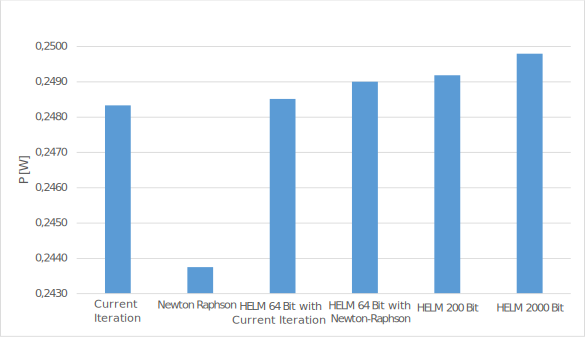
\includegraphics[scale=0.7]{figures/convergence_border}
	\caption{Convergence border for \figref{convergence_border_net}}
	\label{fig:convergence_border}
\end{figure}

To be able to evaluate \emph{HELM} in detail, also for critical nets, which can not be calculate with the iterative methods, I decided to implement \emph{HELM} with the possibility of a configurable precise datatype. As the generics in \emph{C\#} did not gave me the ability to use a library of precise datatypes together with a package for linear algebra I decided to swith for this part of application to \emph{C++}. In this language I had templates available, which allowed the combination of \emph{MPIR}, a library for multi precision integers and rationals, with \emph{Eigen}, a library for sparse linear algebra. Through this I was able to reduce the necessity to reimplement one of these essentials and complex moduls.

\subsection{Linear Algebra}
All the implemented methods have one thing in common: linear algebra. In every method it is necessary to solve linear equation systems, although the equation systems differ in their properties. In \emph{HELM} and the \emph{Current Iteration} the system matrix is the admittance matrix, in \emph{Newton-Raphson} and \emph{FDLF} it is a Jacobian matrix. Both types of matrices are typically sparse, therefore the use of sparse linear algebra improves the performance of the algorithms significantly.

To solve these linear equation systems for instance with a LU-factorization is for big power nets unpractical, as only this step might take hours on current hardware. The solution to this is to use iterative solvers like \emph{BiCGSTAB} \cite{bicgstab}.

The last important detail of the implementation of the calculation methods is the preconditioning. With this step special properties of the system matrix can be used to improve the condition of the equation system and therefore accelerate the iterative solvers. Fortunately, the admittance matrix, which is the system matrix in the \emph{Current Iteration} and \emph{HELM} is approximately diagonal dominant. This makes the application of a diagonal preconditioner very practical, as such a preconditioning is very efficient to calculate and improves the condition of the equation system significantly in this situation.

\section{Link to PSS SINCAL}
\label{sec:link_sincal}